\documentclass[tikz, border=3mm]{standalone}
\usepackage{tikz}
\usetikzlibrary{arrows.meta, decorations.markings, angles, quotes, calc, positioning}

\begin{document}
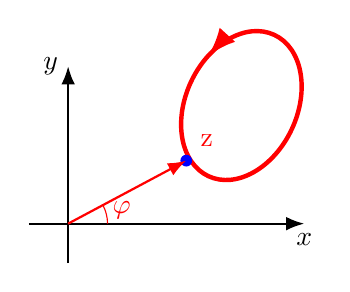
\begin{tikzpicture}[
    >=Latex, % Set default arrow tip style
    path/.style={red, thick}, % Style for the path and vector
    dot/.style={fill=red, circle, inner sep=1.5pt}, % Style for point z
    labelstyle/.style={red} % Style for labels
]

    \coordinate (Ce) at (2.2, 1.5); % Center of the ellipse


    % Axes
    \draw[->, thick] (-0.5, 0) -- (3, 0) node[below] {$x$};
    \draw[->, thick] (0, -0.5) -- (0, 2) node[left] {$y$};

    % Define origin and point z
    \coordinate (O) at (0,0);
    \coordinate (z) at (1.5, 0.8); % Estimated position of z

    % Define ellipse parameters (centered slightly offset from z)
    \coordinate (ellipse_center) at ($(z)+(0.7,0.7)$); % Center near z
    \def\xrad{{sqrt{0.98}}} % x-radius
    \def\yrad{0.5*sqrt(0.98)/0.7} % y-radius
    \def\rotangle{65} % Estimated rotation angle in degrees


    % Draw the red closed curve (ellipse) with arrow
   % draw[path,
    %    postaction={decorate, decoration={markings, mark=at position 0.375 with {\arrow{>}}}} % Arrow near top-left
   % ] (ellipse_center) ellipse [x radius=\xrad, y radius=\yrad];


    \draw[red, ultra thick, postaction={decorate, decoration={markings, mark=at position 0.175 with {\arrow{>}}}}] (Ce) ellipse [x radius=\xrad, y radius=\yrad, rotate=\rotangle];

    % Draw point z indicator and label
    \node[dot, blue, label={[labelstyle]above right:z}] at (z) {};

    % Draw vector from origin to z
    \draw[path, ->] (O) -- (z);

    % Draw angle phi
    \coordinate (xaxis_ref) at (1,0); % Reference point on positive x-axis
    \pic [draw, labelstyle, angle radius=0.5cm, "$\varphi$", angle eccentricity=1.4] {angle = xaxis_ref--O--z};

\end{tikzpicture}
\end{document}